\subsection{Fit results}
\label{sec:FitResults}

Table \ref{tab:FitParams} shows the measured values for the extracted radii and scattering parameters, along with statistical and systematic error bars.
The "Fit Sys" and "Cut Sys" columns list the systematic uncertainties arising from variation in the fit method and in the topological and pair cut values, respectively.
In almost all cases, the cut systematics are an order of magnitude smaller than the fit method systematics.
The "Total Sys" column shows the fit method and cut systematics added in quadrature.
%While the systematic uncertainties are not directly correlated with the statistical uncertainties, 


\begin{table}
\begin{center}

\begin{tabular}{|l|l|l|l|l|l|}
\hline 
Parameter & Value (fm) & $\pm$ Stat & $\pm$ Total Sys & Fit Sys & Cut Sys \\ 
\hline 
Radius $\Lambda\bar{\Lambda}$ 0-10\% & 2.9 & 0.3 & 0.3 & 0.3 & 0.02 \\ 
\hline 
Radius $\Lambda\bar{\Lambda}$ 10-30\%  & 2.3 & 0.2 & 0.2 & 0.2 & 0.02 \\ 
\hline 
Radius $\Lambda\bar{\Lambda}$ 30-50\%  & 1.8 & 0.2 & 0.2 & 0.2 & 0.01 \\ 
\hline 
Radius $\Lambda\Lambda$ 0-10\% & 5.4 & 0.6 & 0.2 & 0.2 & 0.1 \\ 
\hline 
Radius $\Lambda\Lambda$ 10-30\% & 4.2 & 0.5 & 0.2 & 0.2 & 0.04 \\ 
\hline 
$\Re f_0$ $\Lambda\bar{\Lambda}$ & -0.5 & 0.1 & 0.1 & 0.1 & 0.01 \\ 
\hline 
$\Im f_0$ $\Lambda\bar{\Lambda}$ & 0.14 & 0.09 & 0.02 & 0.02 & 0.006 \\ 
\hline 
$\Re f_0$ $\Lambda\Lambda$ & -0.6 & 0.3 & 0.05 & 0.04 & 0.02 \\ 
\hline 
$d_0$ $\Lambda\bar{\Lambda}$ & 1.7 & 0.2 & 0.2 & 0.2 & 0.01 \\ 
\hline 
$d_0$ $\Lambda\Lambda$ & 5.3 & 2.7 & 0.3 & 0.2 & 0.2 \\ 
\hline 
\end{tabular} 
\end{center}
\caption[Fit results]{Measured fit parameters with statistical and systematic errors.
All values are measured in fm.
The Fit Sys and Cut Sys columns show the systematic uncertainties arising from variations in the fit method and the topological and pair cut parameters, respectively.
The Total Sys column comes from the fit and cut systematic errors added in quadrature. }
\label{tab:FitParams}
\end{table}






%\subsubsection{Discussion of results}
%\label{sec:ResultsDiscussion}



\subsubsection{$\Re f_0$}
\label{sec:Ref0Result}


Figure \ref{fig:Ref0} shows the measured $\Re f_0$ for $\Lambda\Lambda$ and $\Lambda\bar{\Lambda}$. A number of other measurements are included for comparison. From the left: $\Lambda\bar{\Lambda}$ and $\Lambda\Lambda \oplus \bar{\Lambda}\bar{\Lambda}$ scattering lengths from this analysis, $\Lambda\Lambda \oplus \bar{\Lambda}\bar{\Lambda}$ from Au--Au $\sqrt{s_{\mathrm{NN}}} = 200\ \mathrm{GeV}/c$ measured at STAR \cite{Adamczyk:2014vca}, $\Lambda\Lambda$ result from a 4-body cluster model of hypernuclear interactions \cite{Hiyama:2002yj} applied to a measurement of $\ce{^{6}_{\Lambda\Lambda}\mathrm{He}}$ \cite{Takahashi:2001nm}, $\Lambda\Lambda$ result from the Nijmegen D soft-core interaction model \cite{Filikhin:2002wm} (also applied to \cite{Hiyama:2002yj}), $\mathrm{p}\bar{\Lambda}$ extracted from a residual correlation analysis \cite{Kisiel:2014mma} of STAR data, $\mathrm{p}\Lambda$ singlet and triplet scattering lengths \cite{Wang:1999bf}, np singlet and triplet scattering lengths \cite{LANDAU1977502}, and the nn scattering length \cite{vonWitsch:1979uni}.

\begin{figure}[hbtp]
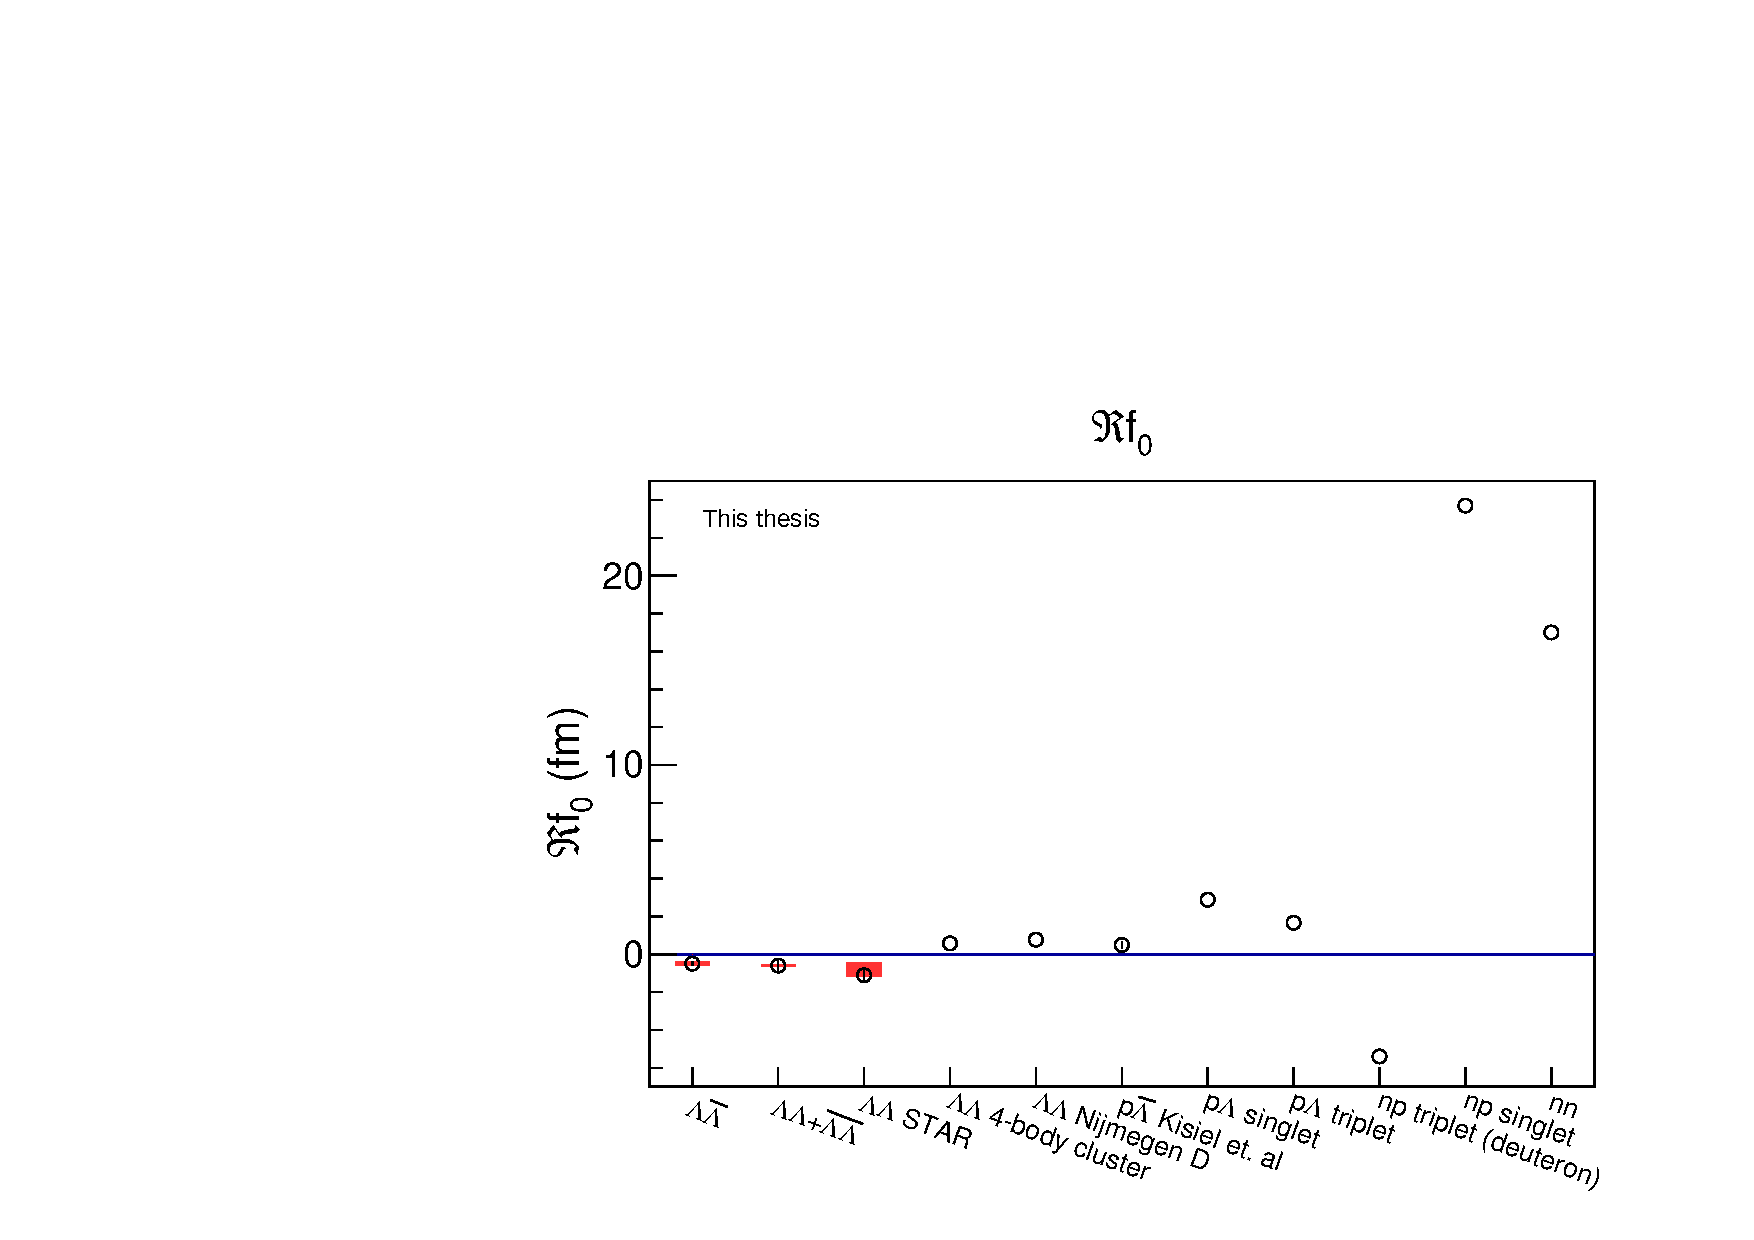
\includegraphics[width=36pc]{Figures/FitResults/2016-10-12-Ref0.pdf}
\caption[Measurements of $\Re f_0$ for various particle pairs]{Several measurements of the real part of the $\Lambda\Lambda$ and $\Lambda\bar{\Lambda}$ scattering lengths. p$\Lambda$, p$\bar{\Lambda}$, np, and nn are included for comparison. The np spin-triplet state --- the deuteron --- is a weakly bound state. The $\Lambda\Lambda$ scattering length is an order of magnitude smaller than the np scattering length, which is evidence that there is no $\Lambda\Lambda$ dibaryon bound state.}
\label{fig:Ref0}
\end{figure}

The np triplet spin state is a known bound state --- the ground state of the deuteron.
 The $\Lambda\Lambda$ scattering length ($\sim-0.6$ fm) is about an order of magnitude smaller than the deuteron scattering length.
Since the deuteron is only weakly bound, the significantly smaller scattering length of $\Lambda\Lambda$ suggests that it does not have a dibaryon bound state.

% Zoomed in picture of the scattering lengths
\begin{figure}[hbtp]
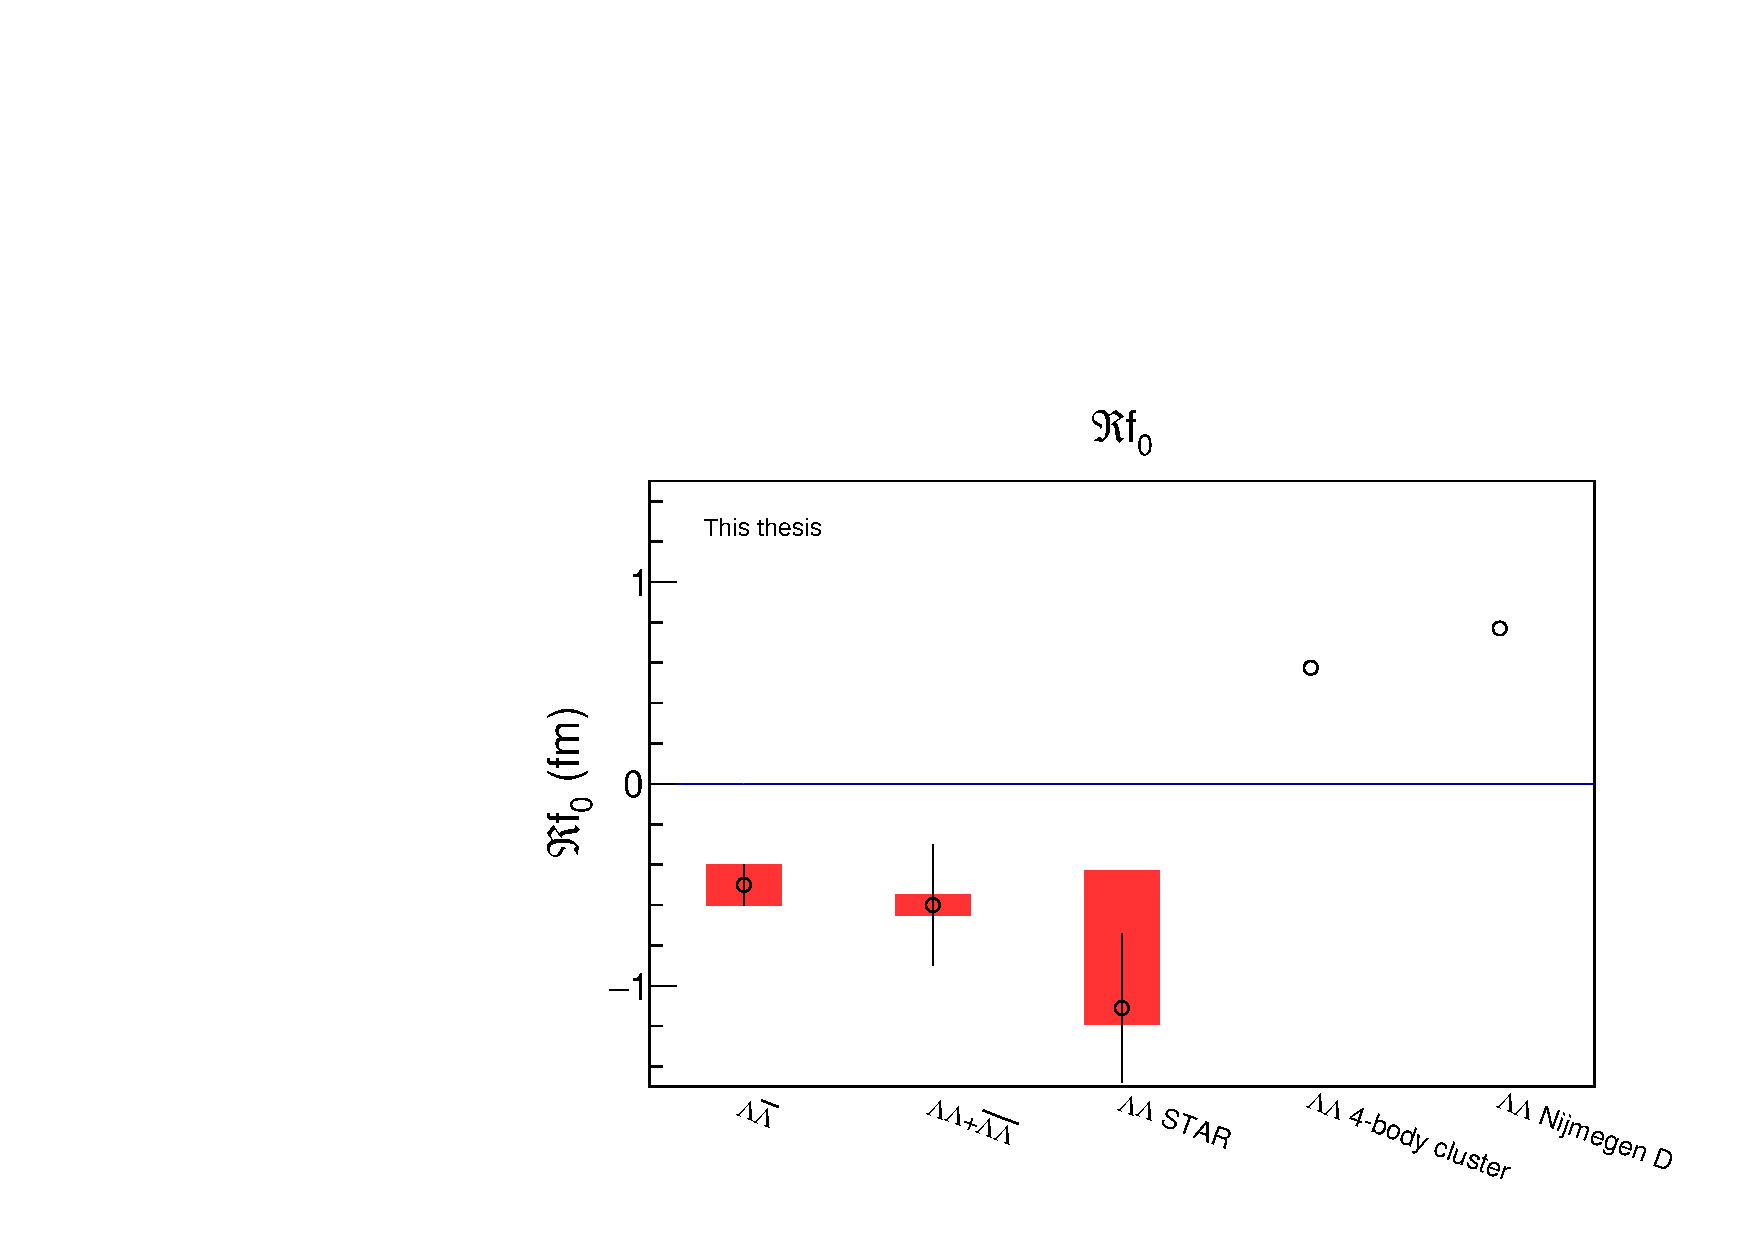
\includegraphics[width=36pc]{Figures/FitResults/2016-10-12-Ref0Zoom.pdf}
\caption[Measurements of $\Re f_0$ for various particle pairs (zoomed)]{Several measurements of the real part of the $\Lambda\Lambda$ and $\Lambda\bar{\Lambda}$ scattering lengths. The STAR measurement \cite{Adamczyk:2014vca} of the $\Lambda\Lambda$ scattering length agrees with our measurement within their systematic uncertainty. Our measurement is similar in magnitude but opposite the sign of $\Lambda\Lambda$ scattering lengths calculated from hypernuclear structure models \cite{ Hiyama:2002yj, Filikhin:2002wm} applied to a measured $\ce{^{6}_{\Lambda\Lambda}\mathrm{He}}$ nucleus \cite{Takahashi:2001nm}.}
\label{fig:Ref0Zoom}
\end{figure}

Figure \ref{fig:Ref0Zoom} shows $\Re f_0$ again, but here it is zoomed in to better highlight the details of the various $\Lambda\Lambda$ measurements.
We can see that the STAR measurement of $\Lambda\Lambda$ agrees with our measurement within their systematic uncertainties.
Our measurement does not agree with the results from the hypernuclear interaction models - they have opposite signs, though similar magnitudes. 



% Discussion of other LA measurement...



%  comparison with LL


\subsubsection{$\Im f_0$}
\label{Imf0Result}


The few measured baryon-antibaryon scattering lengths have imaginary components on the order of 1 fm.
The imaginary part of the $\mathrm{p\bar{p}}$ scattering length has been measured to be $\Im f_{0,\mathrm{p\bar{p}}} = 0.95 \pm 0.12$ fm, and the value for $\mathrm{p\bar{n}}$ is $\Im f_{0,\mathrm{p\bar{n}}} = 0.83 \pm 0.07$ fm \cite{Mutchler:1988av}. 
Analysis of the STAR $\mathrm{p\bar{\Lambda} \oplus \bar{p}\Lambda}$ correlation functions in 200 GeV Au--Au \cite{Adams:2005ws} collisions with (without) accounting for residual correlations yields $\Im f_{0,\mathrm{p\bar{\Lambda}}} = 0.82 \pm 0.28$ fm ($\Im f_{0,\mathrm{p\bar{\Lambda}}} = 1.00 \pm 0.21$ fm) \cite{Kisiel:2014mma}.
It has been hypothesized that all baryon-antibaryon pairs have similar annihilation cross sections at comparable relative momentum \cite{Kisiel:2014mma}.
Indeed, as many $\mathrm{B\bar{B}}$ interactions are unknown, the UrQMD model treats all annihilation cross-sections as being the same as the $\mathrm{p\bar{p}}$ annihilation cross-section at the same $\sqrt{s}$ \cite{Bleicher:1999xi}.

In contrast with these various measurements and models, our measured scattering length is $\Im f_{0,\Lambda\bar{\Lambda}} = 0.14 \pm 0.09\ (\mathrm{stat}) \pm 0.02\ (\mathrm{sys})$ fm.

\subsubsection{$d_0$}
% d0

$d_0$ enters into the wave function as a correction to the scattering amplitude, and in general it has a less profound affect on the correlation function than the scattering length.
There are a few different treatments of $d_0$ across the field of research.
When the value is known, such as for pp femtoscopy \cite{Adam:2015vja}, it implemented as a fixed value in the fits.
In other cases, it has been set to zero to reduce the number of free fit parameters and avoid over-fitting \cite{Kisiel:2014mma, Shapoval:2014yha, Adams:2005ws}.
In this analysis as well as the the STAR analyses of $\bar{\mathrm{pp}}$ and $\Lambda\Lambda$ correlations \cite{Adamczyk:2015hza, Adamczyk:2014vca}, $d_0$ is left as a free parameter with the goal of letting nature tell whatever story it wants to tell.

The moral of that story seems to be that $d_0$ is not very well constrained. 
STAR measured $d_{0,\bar{\mathrm{p}}\bar{\mathrm{p}}} = 2.14\ \mathrm{fm} \pm 0.27\ \mathrm{(stat)} \pm 1.34\ \mathrm{(sys)}$ --- about 60\% uncertainty --- and $d_{0,\Lambda\Lambda} =  8.52\ \mathrm{fm} \pm 2.56\ \mathrm{(stat)}^{+2.09}_{-0.74}\ \mathrm{(sys)}$ --- about 30--40\% uncertainty.
We obtained $d_{0,\Lambda\Lambda} =  5.3\ \mathrm{fm} \pm 2.7\ \mathrm{(stat)} \pm 0.3\ \mathrm{(sys)}$ --- about 50\% uncertainty.
For $\Lambda\bar{\Lambda}$, we faired better with 17\% uncertainty: $d_{0,\Lambda\bar{\Lambda}} =  1.7\ \mathrm{fm} \pm 0.2\ \mathrm{(stat)} \pm 0.2\ \mathrm{(sys)}$.






\subsubsection{Radii}

Figure \ref{fig:RvsMt} shows the extracted 1D radius $R_{\mathrm{inv}}$ for $\Lambda\Lambda\oplus\bar{\Lambda}\bar{\Lambda}$ and $\Lambda\bar{\Lambda}$ as a function of centrality and the average transverse mass $m_{\mathrm{T}}$ of the measured pairs.
Also included are the radii for $\pi^\pm\pi^\pm$, $\mathrm{K^\pm}\mathrm{K^\pm}$, $\mathrm{K^0_S}\mathrm{K^0_S}$, pp, $\bar{\mathrm{p}}\bar{\mathrm{p}}$ \cite{Adam:2015vja}, and p$\Lambda\oplus\bar{\mathrm{p}}\bar{\Lambda}$ (unpublished).
The $\Lambda\bar{\Lambda}$ points seem to follow the $m_\mathrm{T}$ scaling of the pions, kaons, and protons.
The $\Lambda\Lambda$ and p$\Lambda$ radii are quite large, however, and while they are consistent with each other, they do not follow the $m_\mathrm{T}$ scaling trend.
We do not yet have a good explanation of this phenomena.
Nor can we explain why the $\Lambda\Lambda\oplus\bar{\Lambda}\bar{\Lambda}$ and $\Lambda\bar{\Lambda}$ radii are so different.


\begin{figure}[hbtp]
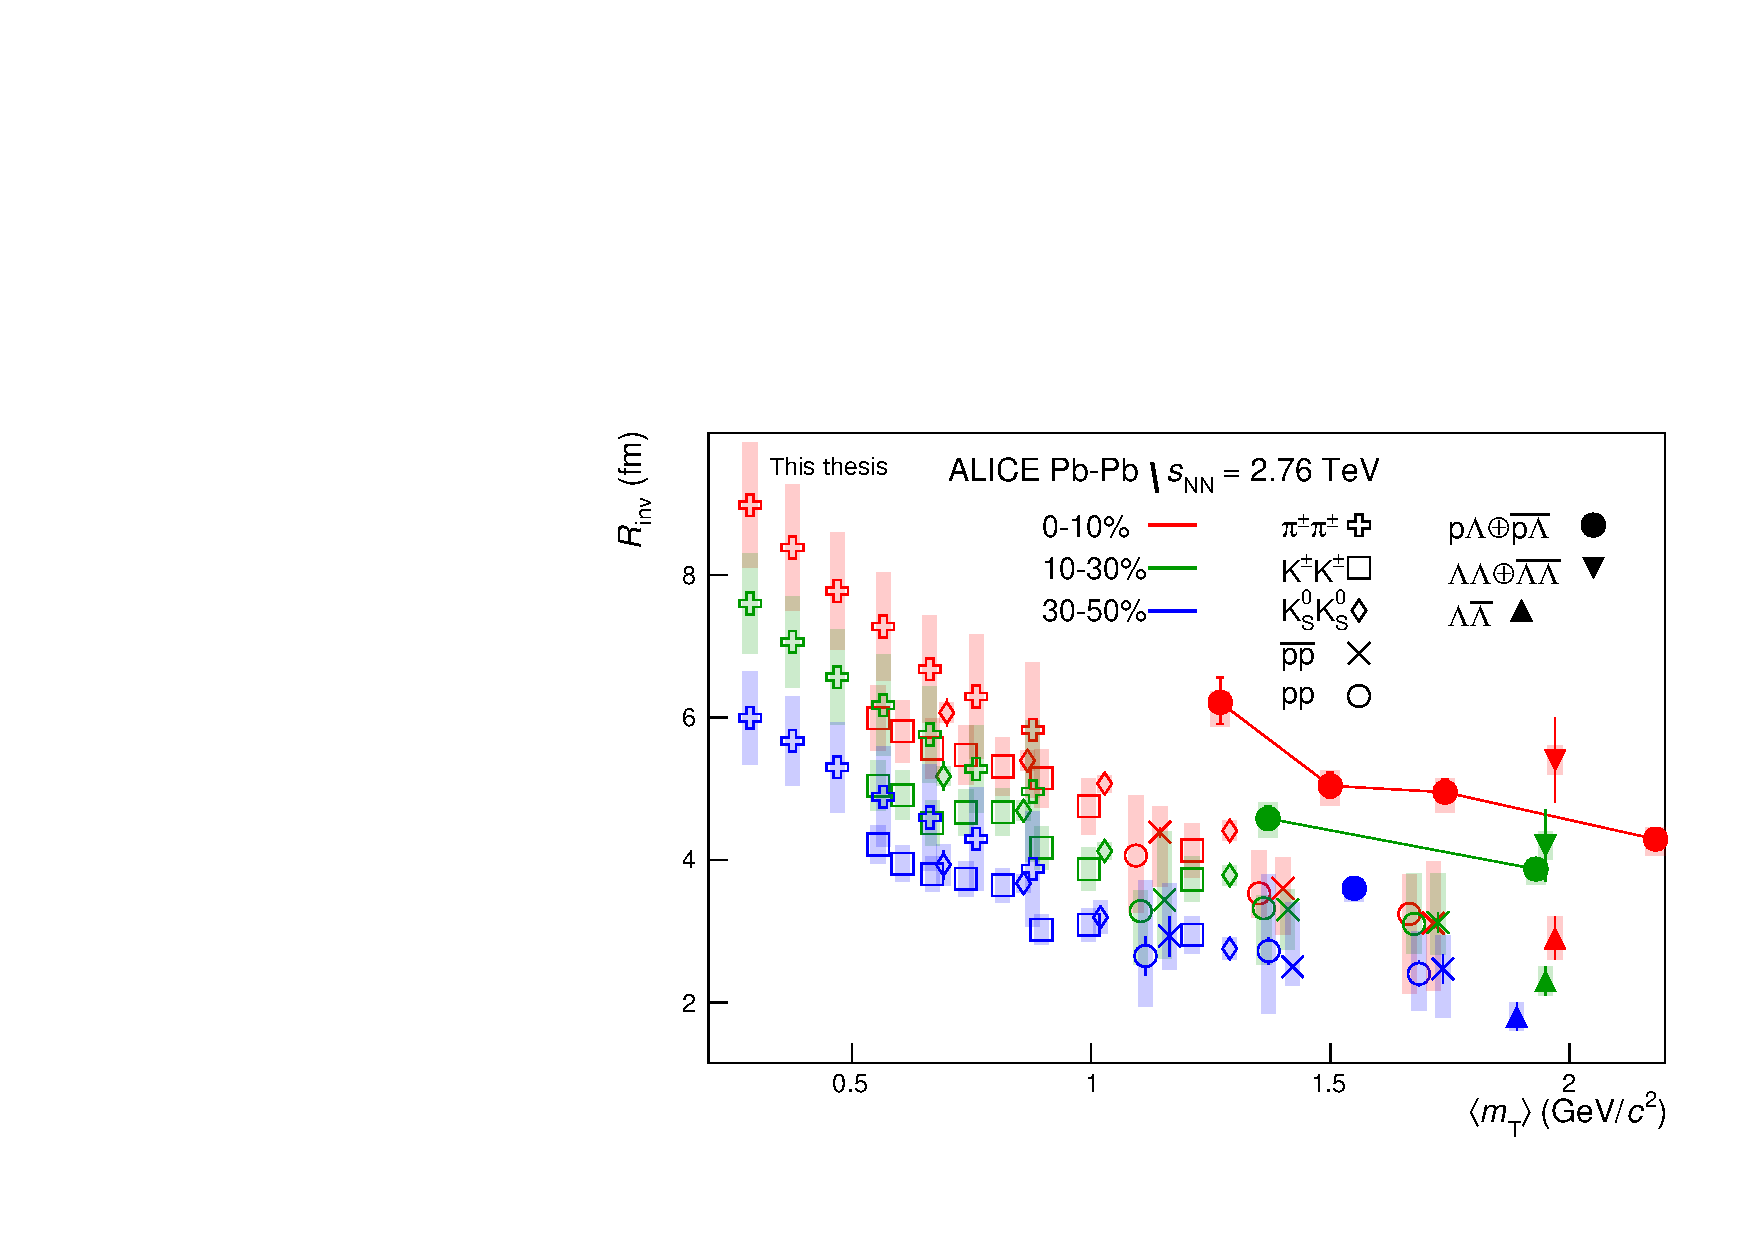
\includegraphics[width=36pc]{Figures/FitResults/2016-09-29-mTscaling.pdf}
\caption[$R_{\mathrm{inv}}$ vs $m_{\mathrm{T}}$]{1D radius $R_\mathrm{inv}$ vs transverse mass $m_\mathrm{T}$ for many different pairs measured by ALICE in $\sqrt{s_\mathrm{NN}} = 2.76$ TeV Pb-Pb collisions \cite{Adam:2015vja}.
The $\Lambda\bar{\Lambda}$ radii appear to follow the trend of $m_\mathrm{T}$-scaling \cite{Csorgo:1995bi,Lisa:2005dd}, but $\Lambda\Lambda\oplus\bar{\Lambda}\bar{\Lambda}$ and $\mathrm{p}\Lambda\oplus\bar{\mathrm{p}}\bar{\Lambda}$ do not.
}
\label{fig:RvsMt}
\end{figure}


% Plot with STAR radii

